\section{System Design: Training–Rollout Decoupling}

\begin{figure}[htb]
  \centering
  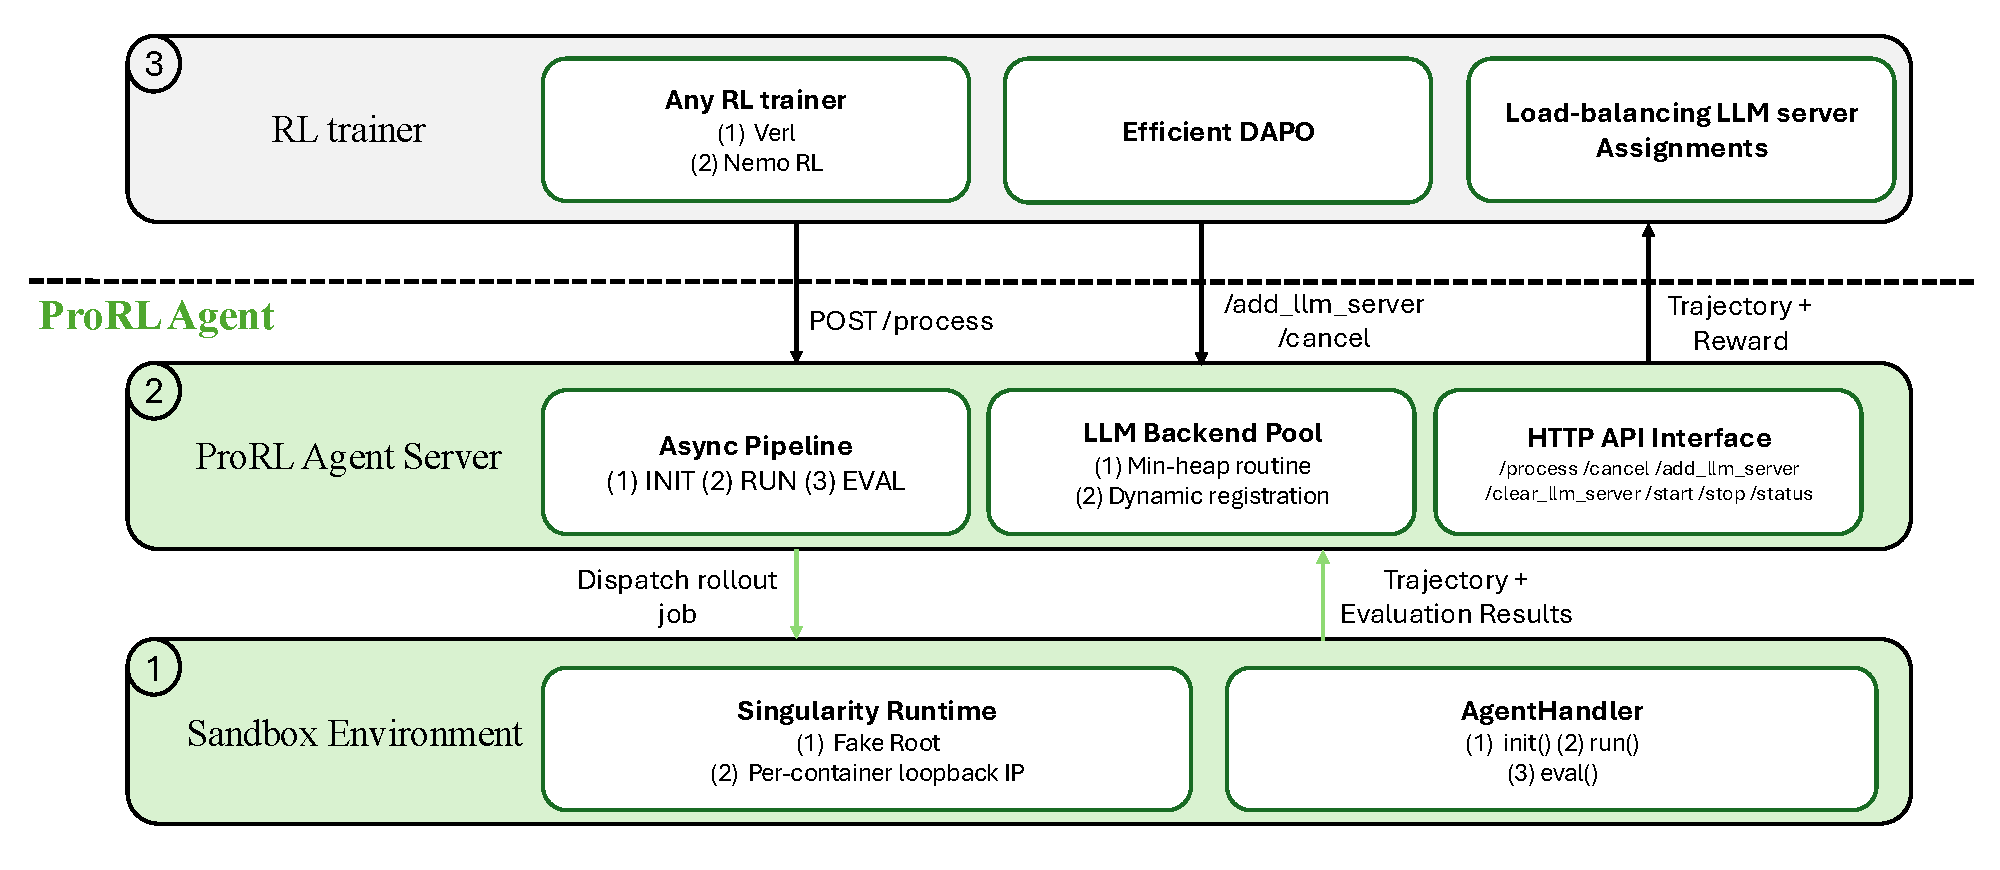
\includegraphics[width=1.0\linewidth]{figures/system_design.pdf}
  \caption{Overview of the \prorlagent architecture. The system consists of three components. 
  \textbf{(1) Sandbox Environment}: each rollout is executed inside a \texttt{SingularityRuntime} container and orchestrated via \texttt{AgentHandler}, which exposes three lifecycle methods including \texttt{init()}, \texttt{run()}, and \texttt{eval()} for environment setup, multi-turn agent execution, and reward scoring, respectively. 
  \textbf{(2) ProRL Agent Server}: an HTTP service that manages rollouts through a three-stage asynchronous pipeline (INIT~$\to$~RUN~$\to$~EVAL) with independent worker pools, and maintains a min-heap LLM backend pool supporting dynamic registration and checkpoint swapping. 
  \textbf{(3) RL Trainer}: any training framework (e.g., veRL, NeMo RL) interacts with the server solely via HTTP, submitting jobs via \texttt{POST \/process} and managing backends via \texttt{\/add\_llm\_server} and \texttt{/cancel}; completed trajectories and rewards are returned to the trainer to update the policy.}
  \label{fig:system_design}
\end{figure}

\subsection{Overview}
\label{sec:overview}

Training RL agents on agentic tasks normally involves multi-turn interaction with live execution environments, where each data sample spans sandbox environment setup, tool execution, and outcome scoring, a process far more complex than single-step generation.
Prior systems typically embed rollout logic directly inside the training loop~\citep{cao2025skyrlagent}, tightly coupling the agent task loop, execution environment, and RL algorithm.
This coupling imposes significant engineering overhead when switching task, and RL trainers.

\prorlagent addresses this through a rollout-as-a-service design with \textbf{rollout-level decoupling}, in which rollout orchestration is fully separated from the training process.
In particular, ProRL Agent Server runs as a standalone HTTP service that accepts a task instance, executes the full agent rollout internally, and returns a completed trajectory with a reward signal. The training framework interacts with the server only through this interface, remaining agnostic to RL infrastructure. This decoupling has three practical consequences.
\begin{itemize}
    \item The RL trainer and agentic rollout logic can be developed, deployed independently: rollout nodes and training nodes can be optimized seperately for larger throughput.
    \item Adding a new task requires only implementing a handler plugin on the rollout server side, with no changes to the training code.
    \item Agentic scaffolds can be modified or replaced without affecting the training infrastructure, as the rollout service and the agent implementation are fully decoupled. 
\end{itemize}
Figure~\ref{fig:system_design} illustrates the overall architecture, which consists of three main components: extensible sandbox environments, the ProRL Agent server for rollout scheduling, and the RL training backend. We introduce each component in turn and describe how they interact within the system.

\subsection{Extensible Sandbox Environments} 
\label{sec:sandbox}

Performing RL training over diverse multi-turn agentic tasks normally requires a sandbox layer that can accommodate heterogeneous task environments and run portably on HPC clusters without privileged access.
We build such the sandbox system around two components: a pluggable task abstraction that decouples task-specific logic from the server core, and an HPC-compatible container runtime that enables isolated, rootless agentic tasks execution at scale.

\subsubsection{Pluggable Task Abstraction}
\label{sec:handlers}

Different agentic tasks e.g., software engineering, mathematical reasoning, computer use, each require their own environment setup, agent behavior, and reward computation.
Hardcoding these differences in the server would make it brittle and always rely on great human efforts.
Instead, we encapsulate all task-specific logic in an abstract interface called \emph{AgentHandler}, which defines three core lifecycle methods corresponding to the three pipeline stages:

\begin{itemize}
  \item \texttt{init}: initialize the sandbox environment for the task, configures the agent with corresponding toolset.
  \item \texttt{run}: drives the multi-turn agent loop within the prepared sandbox environment, collecting the action-observation trajectory and any task artifacts.
  \item \texttt{eval}: scores the agent's output against the ground truth and returns a scalar reward signal for subsequent RL training.
\end{itemize}

Each handler additionally exposes per-stage error callbacks (\texttt{init\_exception}, \texttt{run\_exception}, \texttt{eval\_exception}) and a \texttt{final\_result} method for response serialization, ensuring the server always emits a well-formed output even when a rollout fails partway through.
Listing~\ref{lst:handler} illustrates the interface and a minimal registration example.

\begin{lstlisting}[
  style=pythonstyle,
  caption={The \texttt{AgentHandler} interface and task registration. Each task domain subclasses \texttt{AgentHandler} and registers under a unique name. The server dispatches incoming jobs by matching with different registry.},
  label={lst:handler}
]
class AgentHandler(ABC):
    @abstractmethod
    async def init(self, job_details) -> (Runtime, Metadata, Config):
        """Provision environment; return (runtime, metadata, config)."""
    @abstractmethod
    async def run(self, job_details) -> dict:
        """Execute agent loop; return trajectory and artifacts."""
    @abstractmethod
    async def eval(self, job_details) -> dict:
        """Score output; return reward signal."""
    # Error callbacks (one per stage) and result serializer
    def init_exception(self, job_details, exc) -> dict: ...
    def run_exception(self, job_details, exc)  -> dict: ...
    def eval_exception(self, job_details, exc) -> dict: ...
    def final_result(self, job_details)        -> dict: ...
\end{lstlisting}

When the server receives a job, it reads the task instance, looks up the corresponding handler in the registry, and dispatches to its lifecycle methods in order.

\subsubsection{HPC-Compatible Container Runtime}
\label{sec:runtime}

Most agentic sandbox environments assume a cloud or workstation environment where Docker is readily available.
HPC clusters, however, typically forbid Docker daemons for security reasons, requiring all user processes to run without root privileges under a batch scheduler such as Slurm.
To bridge this gap, we implement \emph{SingularityRuntime}, a container system that requires no persistent daemon and runs entirely as an unprivileged user process to serve sandbox environments.  

\textbf{Container isolation and port management.} 
Each container is launched as a child process in its own session; shutdown proceeds gracefully via \texttt{SIGTERM} before escalating to \texttt{SIGKILL} if necessary.
To support many concurrently running containers on the same node without port conflicts, each container instance is assigned a unique loopback IP address within the \texttt{127.x.x.x} range via a thread-safe allocator.
Two flags address common HPC constraints: \texttt{--fakeroot} grants the container simulated root access for package installation without requiring actual host privileges, and \texttt{--network none} optionally disables external network access to isolate rollouts from interference.

\textbf{Image build pipeline.} 
Container images are packaged as Singularity Image Files (.sif), which encapsulate the full execution environment in a single portable file. This format is particularly well-suited to Slurm shared filesystems, where no persistent container daemon is available.
A companion \texttt{SingularityRuntimeBuilder} constructs images from Jinja2 templates and supports three caching modes: 
\textsc{Scratch} always performs a full rebuild; \textsc{Versioned} reuses a cached image when the base image and framework version are unchanged; and \textsc{Lock} reuses it whenever the dependency lockfile is identical.
The template-driven design enables flexible specialization of runtimes for heterogeneous agentic environments.
For example, QEMU-based virtual machines used in GUI-centric tasks can provide custom definition files to the builder without requiring any modifications to the core build logic.

\subsubsection{Efficient tool backends}
The agent mostly interacts with the environment through tools: it reads and writes files, executes shell commands, runs Python code, and browses the web.
Each tool call is a synchronous blocking operation from the agent's perspective, the agent must wait for the observation before it can decide its next action.
Because a typical rollout spans dozens of such calls, per-tool latency compounds directly into total rollout time, and at high concurrency this overhead can dominate LLM inference as the primary bottleneck.
We therefore optimize three critical tool backends.

\textbf{Efficient Bash.}
Shell execution is the most frequent action across all code-centric agentic tasks. 
Conventional implementations route bash commands through a tmux session, incurring the overhead of terminal multiplexing.
We replace this with a \texttt{ptyprocess}-based direct pseudo-terminal, which grants the agent a raw shell without the tmux intermediary, yielding a significant reduction in shell command round-trip latency.

\textbf{IPython.}
When an agent writes and executes Python code across multiple steps, it is often building on its own prior work: importing a library once, then using it repeatedly; defining a helper function, then calling it later.
A persistent IPython kernel makes this natural so that variables and imports defined in one step remain available in subsequent steps, so the agent does not need to repeat setup code on every call.
The conventional way to host such a kernel is through the Jupyter kernel gateway, but this adds a network round-trip even when the kernel runs on the same machine as the agent.
We instead connect to the kernel directly via its in-process API, removing this overhead entirely. 

\textbf{UDS communication.}
When the agent decides to take an action, such as running a shell command, editing a file, or executing Python, that action is not run directly by the agent process.
Instead, it is sent to a small execution server running inside the container, which carries out the action and sends the observation back.
The common transport for this channel is TCP loopback, which works correctly but forces co-located processes that share the same IP to be distinguished only by port numbers, complicating non-conflicting port assignment and it typically offers lower throughput than Unix domain sockets.
We replace it with Unix domain sockets (UDS), a simpler IPC mechanism that passes messages through the OS kernel directly without any networking overhead. Since this channel is exercised on every agent action, shaving latency here accumulates meaningfully across a full rollout. 

Together, these three optimizations ensure that tool execution does not become the throughput bottleneck as rollout concurrency scales to hundreds of parallel agents.

\subsection{ProRL Agent Server}
\label{sec:server}

With the sandbox layer handling individual rollout execution, the server's
core responsibility during RL training is to orchestrate hundreds of such
rollouts concurrently while providing the training framework with live control
over the rollout infrastructure.

There are two basic requirements for the server:
\begin{itemize}
    \item First, the three rollout phases have fundamentally different resource demands: container initialization is I/O-bound, agent execution is LLM-inference-bound, and outcome evaluation ranges from a few milliseconds for direct scoring to several minutes for full test-suite execution. Executing these phases within each job should not limit throughput to the slowest stage.
    \item Second, the training framework needs dynamic control over LLM inference backends: it must be able to register new servers as the compute cluster scales, swap backends when model checkpoints are updated, and cancel stale in-flight jobs whose gradient batch has already advanced, all without tight coupling to the server internals. 
\end{itemize}

ProRL Agent Server addresses both facets through two mechanisms: 
\textbf{(1) An asynchronous three-stage pipeline} that assigns each rollout phase to an independent worker pool so all three phases can overlap across the job population; and 
\textbf{(2) A lightweight management API} that exposes job submission, per-job cancellation, LLM backend registration, and server lifecycle control to any RL training framework over HTTP.
Listing~\ref{lst:server} sketches the resulting architecture.

\begin{lstlisting}[
  style=pythonstyle,
  label={lst:server},
  caption={Simplified logic of the ProRL Agent Server.  Three independent
           worker pools drain their respective queues concurrently.},
]
# -- Three independent worker pools -------------------------------
STAGES = [INIT, RUN, EVAL]
queues = {s: Queue() for s in STAGES}   # thread-safe FIFO per stage
pools  = {s: ThreadPool(N[s]) for s in STAGES}
llm_backends = MinHeap()                # min-heap keyed by in-flight count

def worker_loop(stage):
    while running:
        job = queues[stage].get()
        if job.id in discarded: continue
        with job.timer.phase(stage):    # only this phase counts toward timeout
            try:
                result = handler[stage](job)
            except Exception as e:
                result = handler[stage+'_exception'](job, e)
        job.store(stage, result)
        if stage == RUN:
            cleanup(job.runtime)        # free container before eval starts
        if stage != EVAL:
            queues[next_stage[stage]].put(job)
        else:
            job.done.set()              # unblock the waiting HTTP handler
\end{lstlisting} 

\subsubsection{Three-Stage Rollout Pipeline}
\label{sec:pipeline}

Think of the rollout process as an assembly line. A naive implementation would assign one worker to each job and have that worker do everything: start the container, run the agent, and score the result, before picking up the next job.
The problem is that each phase takes a very different amount of time and uses a very different resource.
Container startup is slow because it is waiting on disk I/O and the network.  Agent execution is fast per call but fires dozens of LLM requests, so it is bottlenecked by GPU throughput.
Evaluation can be nearly instant for a math answer check, or take several minutes for a full test suite.
A single worker sitting through all three phases in sequence would spend most of its time idle, waiting for whichever phase happens to be slow.

In ProRL Agent server, the solution is to decouple the phases, exactly as a factory decouples assembly stations.
The three lifecycle methods of \texttt{AgentHandler}(Section~\ref{sec:handlers}) map onto three independent worker pools, each with its own queue.
Initialization workers continuously pull new jobs, spin up containers, and hand them off to the rollout queue.
Rollout workers drive agent loops and hand completed trajectories to the evaluation queue.
Evaluation workers score results and return them to the caller. 

At any moment, all three pools are busy on different jobs simultaneously: while one job is being evaluated, a second is mid-rollout, and a third is having its container started.
Because the pools are independent, they can also be sized separately to match their respective workloads, with more init workers to absorb the slow I/O startup, or more eval workers when test suites are particularly long.

\subsubsection{LLM Backend Management}
\label{sec:llm-mgmt}

\begin{lstlisting}[
  style=pythonstyle,
  label={lst:server_api},
  caption={Simplified logic of the ProRL Agent Server. The
           management API gives the training framework full control over jobs
           and LLM backends at runtime.},
]
# -- Management API (HTTP endpoints) -------------------------------
POST /add_llm_server   {"address": "http://host:port/v1"}  # register backend
POST /clear_llm_server                                      # flush all backends
POST /process  {"instance": {...}, "sampling_params": {...}}  # submit job
POST /cancel   {"job_id": "..."}                            # abort running job
POST /start  |  POST /stop                                  # server lifecycle
GET  /status                                                # queue depths
\end{lstlisting}

Every step of the agent loop requires an LLM completion: the model receives the current conversation history and produces the next action.
When hundreds of rollouts run in parallel, these calls arrive at the inference layer simultaneously and at high frequency.
A single LLM server (e.g., vLLM server) quickly becomes a bottleneck, so RL training typically co-deploys a pool of LLM servers and distributes inference traffic across them.
The ProRL Agent Server manages this pool directly, handling both registration and routing so that the training framework does not need to coordinate LLM access itself.

\textbf{Dynamic registration and checkpoint swapping.}
LLM backends are registered and deregistered through the management API at any time during a training run. We show the simplified logic in Listing~\ref{sec:llm-mgmt}
When a new LLM server comes online, the trainer calls \texttt{POST /add\_llm\_server} with the server's endpoint; the server is immediately available for routing.
When the RL trainer updates the policy checkpoint (e.g., after a gradient synchronization step), the old LLM weights are no longer valid.
Rather than restarting the rollout server, the trainer calls \texttt{POST /clear\_llm\_server} to flush all registered backends, then re-registers the reloaded LLM server endpoints.
From that point on, all subsequent rollouts automatically use the updated model, with no interruption to jobs already in the pipeline.


\textbf{Load balancing via min-heap.}
Each LLM backend is stored alongside an assignment counter in a min-heap.
Every time the rollout stage needs to issue an LLM call, ProRL Agent server automatically selects the backend with the lowest counter and assigns that entire task to the selected LLM. The counter is incremented once per task (rather than per call), ensuring that all subsequent calls within the same task are consistently routed to the same backend to maximize prefix cache reuse. After assignment, the backend’s updated counter is used to maintain its position in the heap:
\begin{align*}
  s^{*} = \arg\min_{s}\; w_{s}, \qquad w_{s^{*}} \leftarrow w_{s^{*}} + 1,
\end{align*}
where $w_s$ counts the total number of inference calls assigned to server $s$ since it was registered.
Because selection is proportional to assignment count, servers that receive heavier traffic fall back in priority, achieving a round-robin-like balance across the pool without requiring any global synchronization.
The entire operation is protected by a single lock, making it safe under the high concurrency of the rollout worker pool.


\subsubsection{Token-in/Token-out}
If trajectories are transmitted through the training pipeline as plain text, re-tokenization on the can be lossy: the resulting token sequence may differ from the one originally generated during rollout~\citep{team2025notokenization}, leading to unintended off-policy discrepancies.

\prorlagent eliminates this \emph{re-tokenization drift} by using token IDs as the canonical representation throughout the entire training process.
The rollout worker sends \texttt{prompt\_ids} directly to the LLM backend and receives \texttt{response\_ids} with per-token log-probabilities; each message additionally carries \texttt{input\_ids}, \texttt{output\_ids}, and \texttt{logprobs} fields that are populated at generation time and propagated unchanged.
During multi-turn rollouts, prior assistant turns retain their original token IDs and are concatenated directly into the input buffer; only new messages (e.g., environment observations) are tokenized and appended.
This ensures that every token ID returned to the trainer is identical to the one produced during rollout.

\subsubsection{Job Lifecycle and Cancellation}
\label{sec:lifecycle}

We then describe the lifecycle of each job instance and the cancellation mechanism, which together provide greater flexibility for RL trainers.

\textbf{Phase-aware timeouts.}
Each job is associated with a \texttt{PausableTimer} that accumulates elapsed time only during active pipeline stages (\textit{init}, \textit{run}, and \textit{eval}), while excluding time spent waiting in inter-stage queues. This design ensures that the timeout budget reflects actual execution time rather than transient server-side delays.

\textbf{Cancellation.}
The training framework can abort any in-flight job at any time via \texttt{POST /cancel}.
Once received, ProRL Agent server will: 
(i)mark the job as discarded so that any worker that has not yet dequeued it will skip it; 
(ii)cancel the currently executing async task; 
(iii)close the associated container runtime to release resources immediately; and 
(iv)signal the job's completion event so the waiting HTTP handler returns without blocking.
This enables the RL trainer to discard incomplete rollouts once a sufficient number of valid samples has been collected.

\textbf{Fault isolation.}
Each pipeline stage registers a dedicated exception callback. Once failure, the callback populates \texttt{JobDetails} with a structured fallback result and sets the completion event, preventing any single failed rollout from stalling the shared worker pool.

\textbf{Graceful shutdown.}
Once received \texttt{POST /stop}, the server cancels all in-flight jobs, terminates Singularity processes via process-group scanning, drains the worker pools, and exits cleanly, leaving no orphaned containers on the node.

\begin{figure}[t]
  \centering
  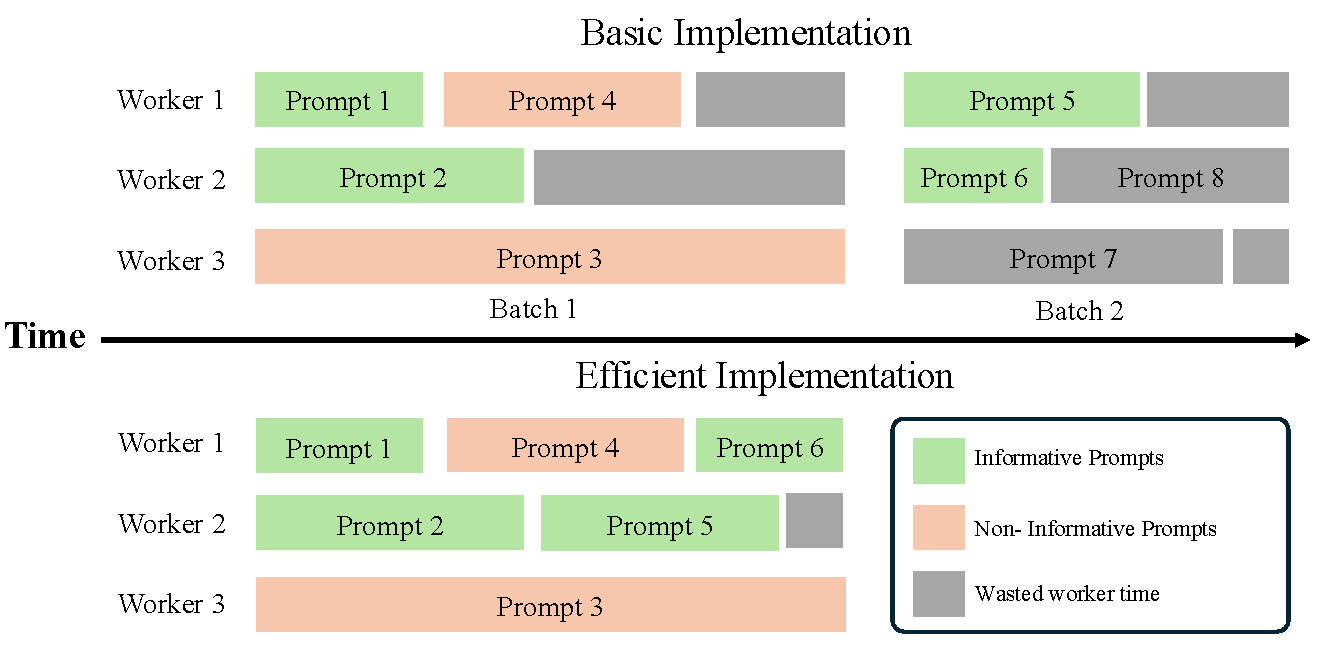
\includegraphics[width=1.0\linewidth]{figures/dapo.pdf}
\caption{Comparison of DAPO implementations ($n=4$). Our efficient implementation optimizes worker synchronization, significantly reducing the idle time (waiting period) between rollout generations compared to the baseline batch-by-batch approach.}
  \label{fig:dapo}
\end{figure}

\subsection{Connecting to RL Trainers}
Rollout-level decoupling allows the agent server to interface with a wide range of RL trainers. In our implementation, we support both VeRL~\cite{sheng2025verl} and NeMo RL~\cite{nemo-rl}. In addition, we provide several key features that further improve RL training.

\textbf{Efficient Asynchronous Task Scheduling.} On the RL client side, we implement a two-phase hierarchical load balancing strategy that jointly optimizes communication locality and global load balance. In the first phase, LLM servers are assigned preferentially to \prorlagent servers on the same physical node, identified through IP address matching, to reduce network latency. In the second phase, any remaining servers are distributed in a round-robin manner to maintain balanced allocation across all available LLM servers.



\textbf{Efficient DAPO.} We adopt Dynamic Sampling Policy Optimization (DAPO)~\citep{yu2025dapoopensourcellmreinforcement} as our core reinforcement learning algorithm. DAPO enhances training stability and data efficiency by filtering out Zero-Variance Prompts—those whose rollouts yield uniform rewards (e.g., all correct or all incorrect) and thus provide no gradient signal. However, applying DAPO to Agent RL is challenging because agent rollouts are typically long-running, asynchronous, and computationally expensive.A naive batch-by-batch implementation—where the trainer requests $n$ prompts, filters out the non-informative ones, and repeatedly triggers new batches until $n$ Informative Prompts are collected—is highly inefficient. This synchronous approach leads to worker idle time and generates redundant rollouts that exceed the target count. Furthermore, discarding incomplete rollouts at the end of a batch results in significant data waste.To address these bottlenecks, we implement an asynchronous replenishment mechanism:
\begin{enumerate}
    \item \textbf{Continuous Throughput:} We replenish the job queue as soon as it empties to maintain maximum rollout throughput.
    \item \textbf{Early Termination:} We terminate remaining active jobs once the target number of Informative Prompts is reached.
    \item \textbf{Cross-Iteration Persistence:} Unfinished jobs are carried over to the subsequent iteration to preserve partial progress.
    
\end{enumerate}
As illustrated in \Cref{fig:dapo}, our optimized implementation significantly reduces worker idle time and improves overall hardware utilization compared to the baseline.  

